% 20-minute project talk, lecture style. Compile: latexmk -pdf presentation.tex
\documentclass[12pt]{beamer}   % 4:3, like the course slides
\usepackage[T1]{fontenc}
\usepackage[scaled=0.95]{helvet}
\usepackage{amsmath,amssymb,booktabs}
\usepackage{tikz,pgfplots}
\pgfplotsset{compat=1.16}
\usetikzlibrary{arrows.meta,patterns,decorations.pathreplacing}

% ---------- colors: dark on white, readable on a projector ----------
\definecolor{navy}{HTML}{0B2545}
\definecolor{orange}{HTML}{F28C00}
\definecolor{red}{HTML}{B3261E}
\definecolor{pale}{HTML}{E3ECF7}
\definecolor{gray}{HTML}{555555}
\definecolor{ink}{HTML}{111111}

% ---------- plain lecture-style theme ----------
\usetheme{default}
\setbeamertemplate{navigation symbols}{}
\setbeamercolor{normal text}{fg=ink,bg=white}
\setbeamercolor{structure}{fg=navy}
\setbeamercolor{block title}{bg=navy,fg=white}
\setbeamercolor{block body}{bg=pale,fg=ink}
\setbeamerfont{block title}{series=\bfseries}
\setbeamerfont{frametitle}{series=\bfseries,size=\Large}
\setbeamertemplate{itemize item}{\color{navy}\rule[0.2ex]{0.9ex}{0.9ex}}
\setbeamertemplate{itemize subitem}{\color{navy}--}
\setbeamersize{text margin left=8mm,text margin right=8mm}
\setbeamertemplate{frametitle}{%
  \vspace{2.5mm}%
  {\color{gray}\small\insertsection\strut\par}%
  {\usebeamerfont{frametitle}\color{navy}\insertframetitle\strut\par}%
  \vspace{0.5mm}{\color{navy}\hrule height 1.3pt}}
\setbeamertemplate{footline}{\hspace{8mm}{\color{gray}\scriptsize Scheduling with declared time limits}\hfill
  {\color{gray}\scriptsize\insertframenumber\,/\,\inserttotalframenumber}\hspace{8mm}\vspace{2.5mm}}

% ---------- helpers ----------
\newcommand{\Opt}{\textsc{Opt}}
\newcommand{\cost}{\mathrm{cost}}
\tikzset{
  lng/.style={fill=navy,draw=white,line width=1.2pt,text=white,font=\bfseries},
  sht/.style={fill=orange,draw=white,line width=1.2pt,text=ink,font=\bfseries},
  ghost/.style={fill=white,draw=navy,dashed,line width=1.2pt,text=navy,font=\bfseries},
  job/.style={draw=navy,fill=pale,line width=1pt,minimum width=1.15cm,minimum height=0.8cm,font=\bfseries},
  mach/.style={fill=navy,text=white,minimum width=2.5cm,minimum height=0.7cm,font=\bfseries},
}
% \gbar{x0}{x1}{y}{style}{label}: a job from time x0 to x1
\newcommand{\gbar}[5]{\draw[#4] (#1,#3) rectangle (#2,#3+0.7) node[pos=.5]{#5};}
% one highlighted statement
\newcommand{\keybox}[2]{\tikz[baseline]\node[fill=pale,draw=navy,line width=1.3pt,inner sep=6pt,align=center]
  {{\color{navy}\bfseries #1} #2};}
% link to a topic of the course
\newcommand{\inclass}[1]{{\small\color{navy}\textbf{In class:} #1}}

\begin{document}

% ======================================================================
\begin{frame}[plain]
  \vspace{12mm}
  {\color{navy}\bfseries\LARGE Online Scheduling of Batch Jobs\\[2pt] with Declared Time Limits\par}
  \vspace{3mm}{\color{navy}\hrule height 1.3pt}
  \vspace{7mm}
  {\large Tianpei Liao \quad and \quad Yiming Shao\par}
  \vspace{3mm}
  {\color{gray}EECS 6111 \ Project presentation\par}
\end{frame}

% ======================================================================
\section{Motivation}

\begin{frame}{Shared compute clusters}
  \centering
  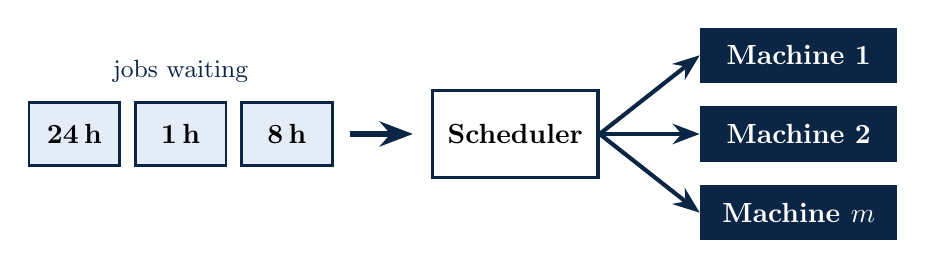
\begin{tikzpicture}[>=Stealth]
    \foreach \x/\l in {0/24\,h,1.35/1\,h,2.7/8\,h} \node[job] at (\x,0) {\l};
    \node[navy,font=\small] at (1.35,0.8) {jobs waiting};
    \draw[->,line width=2pt,navy] (3.5,0) -- (4.3,0);
    \node[draw=navy,line width=1.2pt,fill=white,minimum width=2.1cm,minimum height=1.1cm,font=\bfseries] (s) at (5.6,0) {Scheduler};
    \foreach \y/\l/\n in {1.0/Machine 1/a,0/Machine 2/b,-1.0/Machine $m$/c} {
      \node[mach] (m\n) at (9.2,\y) {\l};
      \draw[->,line width=1.5pt,navy] (s.east) -- (m\n.west);
    }
  \end{tikzpicture}

  \vspace{4mm}
  \begin{itemize}\setlength{\itemsep}{2mm}
    \item<2-> Many users share one cluster: model training, simulations, data pipelines, test builds.
    \item<3-> The \textbf{scheduler} decides which job runs next.
    \item<4-> A bad decision makes many users wait.
  \end{itemize}
\end{frame}

% ======================================================================
\begin{frame}{Jobs come with a time limit}
  \begin{itemize}
    \item<1-> A user submits a job and \textbf{declares a time limit}.
  \end{itemize}
  \vspace{1mm}
  \onslide<2->{
  \centering\small
  \renewcommand{\arraystretch}{1.2}
  \begin{tabular}{ll}
    \toprule
    \textbf{System} & \textbf{The limit} \\
    \midrule
    HPC cluster (Slurm) & \texttt{sbatch -{}-time=8:00:00} \\
    Kubernetes Job & \texttt{activeDeadlineSeconds} \\
    AWS Batch (cloud) & job \texttt{timeout} \\
    GitHub Actions (CI) & \texttt{timeout-minutes} \\
    \bottomrule
  \end{tabular}\par}
  \vspace{2mm}
  \begin{itemize}
    \item<3-> The system \textbf{kills} the job at its limit.
    \item<4-> So users ask for \textbf{more time than they need}.
  \end{itemize}
\end{frame}

% ======================================================================
\begin{frame}{The limit is only an upper bound}
  \centering
  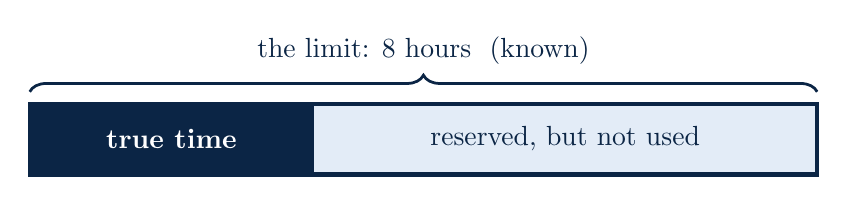
\begin{tikzpicture}[x=1cm,y=1cm]
    \draw[navy,line width=1.5pt,fill=pale] (0,0) rectangle (10,0.9);
    \draw[decorate,decoration={brace,amplitude=6pt},navy,line width=1pt] (0,1.05) -- (10,1.05)
      node[midway,above=6pt] {the limit: 8 hours \ (known)};
    \onslide<2->{
      \draw[fill=navy,draw=navy] (0,0) rectangle (3.6,0.9);
      \node[text=white,font=\bfseries] at (1.8,0.45) {true time};
      \node[navy] at (6.8,0.45) {reserved, but not used};
    }
  \end{tikzpicture}

  \vspace{4mm}
  \begin{itemize}\setlength{\itemsep}{2.5mm}
    \item<2-> The true running time is known \textbf{only when the job ends}.
    \item<3-> On real clusters, the limits are far from the true running times.
          {\small\color{gray}[Mu'alem, Feitelson 2001; Tsafrir et al.\ 2007]}
  \end{itemize}
\end{frame}

% ======================================================================
\begin{frame}{What we study}
  \begin{itemize}\setlength{\itemsep}{3mm}
    \item<1-> The scheduler sees the limits. It does not see the true running times.
    \item<2-> A started job runs to the end. A wrong start cannot be undone.
  \end{itemize}
  \vspace{4mm}
  \onslide<3->{
  \begin{block}{Our question}
    A limit is a weak hint about the length of a job.\\[2pt]
    \textbf{How much can a scheduler gain from it, and how should it use it?}
  \end{block}}
\end{frame}

% ======================================================================
\section{From the real problem to an online problem}

\begin{frame}{The model}
  \small
  \renewcommand{\arraystretch}{1.45}
  \begin{tabular}{@{}ll@{}}
    \toprule
    \textbf{Real cluster} & \textbf{Model} \\
    \midrule
    \uncover<1->{nodes of one cluster} & \uncover<1->{$m$ identical machines} \\
    \uncover<2->{users submit jobs over time} & \uncover<2->{job $j$ arrives at time $r_j$ \ (\textbf{online})} \\
    \uncover<3->{requested time limit} & \uncover<3->{$u_j$, \textbf{known} on arrival} \\
    \uncover<4->{actual running time} & \uncover<4->{$p_j$, \textbf{hidden} until the job ends} \\
    \uncover<5->{limits overestimate} & \uncover<5->{$u_j / \lambda \;\le\; p_j \;\le\; u_j$} \\
    \uncover<6->{no preemption} & \uncover<6->{a started job cannot be stopped} \\
    \bottomrule
  \end{tabular}

  \vspace{3mm}
  \normalsize
  \onslide<5->{$\lambda = 4$: \ the user asks for 8 hours, the job runs 2 to 8 hours.}
\end{frame}

% ======================================================================
\begin{frame}{Objective}
  \begin{block}{Objective}
    Minimize the \textbf{total completion time} \ $\displaystyle\sum_j C_j$\\[2pt]
    $C_j$ = the time when job $j$ finishes
  \end{block}
  \vspace{1mm}
  \begin{itemize}
    \item<2-> Each user cares when \emph{their own} job is done.
  \end{itemize}
  \vspace{1mm}
  \centering
  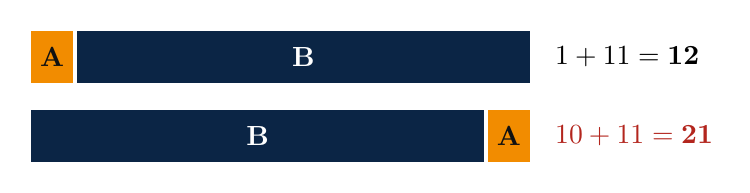
\begin{tikzpicture}[x=0.58cm,y=1cm]
    \onslide<3->{
      \gbar{0}{1}{1.2}{sht}{A}\gbar{1}{11}{1.2}{lng}{B}
      \node[anchor=west] at (11.3,1.55) {$1 + 11 = \mathbf{12}$};
    }
    \onslide<4->{
      \gbar{0}{10}{0.2}{lng}{B}\gbar{10}{11}{0.2}{sht}{A}
      \node[anchor=west,red] at (11.3,0.55) {$10 + 11 = \mathbf{21}$};
    }
  \end{tikzpicture}

  \vspace{1mm}
  \onslide<5->{\textbf{Short jobs should go first.} But which jobs are short?}
\end{frame}

% ======================================================================
\begin{frame}{Competitive ratio for this problem}
  \begin{itemize}\setlength{\itemsep}{3mm}
    \item<1-> The input $\sigma$ is the sequence of jobs. \ $\cost(\sigma) = \sum_j C_j$
    \item<2-> \Opt{} has the same machines and no preemption, but it \textbf{knows all jobs and their true times}.
    \item<3-> $\lambda = 1$: the limits are exact. \ Larger $\lambda$: a weaker hint.
  \end{itemize}
  \vspace{3mm}
  \onslide<4->{
  \begin{block}{Goal of the project}
    The best possible competitive ratio, as a function of $\lambda$.
  \end{block}}
\end{frame}

% ======================================================================
\section{Connection to the course}

\begin{frame}{The simplest setting is bin packing}
  Suppose the running times are known, and all jobs must finish within a time window $T$.
  \vspace{2mm}

  \begin{columns}[c]
    \column{0.45\textwidth}
      \centering
      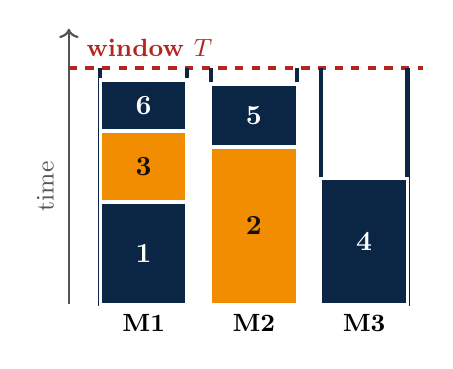
\begin{tikzpicture}[x=1cm,y=1cm]
        \draw[->,thick,gray] (-0.4,0) -- (-0.4,3.5);
        \node[gray,font=\small,rotate=90] at (-0.7,1.5) {time};
        \draw[red,dashed,line width=1.5pt] (-0.4,3) -- (4.1,3);
        \node[red,anchor=south west,font=\small\bfseries] at (-0.3,3.02) {window $T$};
        \foreach \x in {0,1.4,2.8} \draw[navy,line width=1.5pt] (\x,3.0) -- (\x,0) -- (\x+1.1,0) -- (\x+1.1,3.0);
        \onslide<2->{
          \draw[lng] (0,0) rectangle (1.1,1.3) node[pos=.5]{1};
          \draw[sht] (0,1.3) rectangle (1.1,2.2) node[pos=.5]{3};
          \draw[lng] (0,2.2) rectangle (1.1,2.85) node[pos=.5]{6};
          \draw[sht] (1.4,0) rectangle (2.5,2.0) node[pos=.5]{2};
          \draw[lng] (1.4,2.0) rectangle (2.5,2.8) node[pos=.5]{5};
          \draw[lng] (2.8,0) rectangle (3.9,1.6) node[pos=.5]{4};
        }
        \foreach \x/\l in {0.55/M1,1.95/M2,3.35/M3} \node[below,font=\small\bfseries] at (\x,0) {\l};
      \end{tikzpicture}
    \column{0.55\textwidth}
      \onslide<2->{
      \renewcommand{\arraystretch}{1.5}
      \begin{tabular}{@{}l@{\ $=$\ }l@{}}
        machine & bin, capacity $T$ \\
        job & item, size $p_j$ \\
        fewest machines & fewest bins \\
      \end{tabular}}
  \end{columns}

  \vspace{2mm}
  \onslide<3->{\centering\keybox{In class:}{this is online bin packing. First Fit has c.r.\ 1.7.}\par}
\end{frame}

% ======================================================================
\begin{frame}{From bin packing to our problem}
  Three changes:
  \vspace{1mm}
  \begin{enumerate}\setlength{\itemsep}{3.5mm}
    \item<1-> \textbf{$m$ machines are fixed; the cost is $\sum_j C_j$.}\\
          Now the \emph{order} inside a bin matters.
    \item<2-> \textbf{Jobs arrive over time.}\\
          Now we may \emph{wait} before we start a job.\\
          \inclass{ski rental (rent or buy)}
    \item<3-> \textbf{Sizes are hidden; we see only the limits.}\\
          An item may be much smaller than it looks.\\
          \inclass{advice and predictions}
  \end{enumerate}
\end{frame}

% ======================================================================
\section{Opt and known algorithms}

\begin{frame}{Example: four jobs, one machine}
  All four jobs arrive at time 0. \ $\lambda = 4$.
  \vspace{3mm}

  \centering
  \renewcommand{\arraystretch}{1.25}
  \begin{tabular}{c@{\qquad}c@{\qquad}c}
    \toprule
    Job & limit $u_j$ & true time $p_j$ \\
        & (known) & \uncover<2->{{\color{red}(hidden)}} \\
    \midrule
    1 & 8 & \uncover<2->{{\color{red}8}} \\
    2 & 2 & \uncover<2->{{\color{red}1}} \\
    3 & 4 & \uncover<2->{{\color{red}4}} \\
    \textbf{4} & \textbf{8} & \uncover<2->{{\color{red}\textbf{2}}} \\
    \bottomrule
  \end{tabular}

  \vspace{3mm}
  \onslide<3->{Job 4 asks for 8 but needs only 2.}
\end{frame}

% ======================================================================
\begin{frame}{Example: three schedules}
  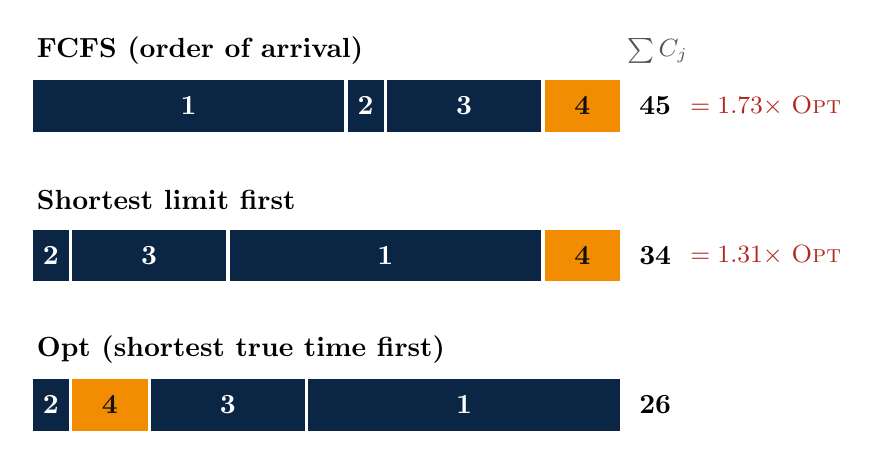
\begin{tikzpicture}[x=0.5cm,y=1cm]
    \node[anchor=west,font=\bfseries] at (-0.1,5.15) {FCFS (order of arrival)};
    \gbar{0}{8}{4.1}{lng}{1}\gbar{8}{9}{4.1}{lng}{2}\gbar{9}{13}{4.1}{lng}{3}\gbar{13}{15}{4.1}{sht}{4}
    \node[anchor=west] at (15.2,4.45) {$\mathbf{45}$};
    \onslide<2->{
      \node[anchor=west,font=\bfseries] at (-0.1,3.25) {Shortest limit first};
      \gbar{0}{1}{2.2}{lng}{2}\gbar{1}{5}{2.2}{lng}{3}\gbar{5}{13}{2.2}{lng}{1}\gbar{13}{15}{2.2}{sht}{4}
      \node[anchor=west] at (15.2,2.55) {$\mathbf{34}$};
    }
    \onslide<3->{
      \node[anchor=west,font=\bfseries] at (-0.1,1.35) {\Opt{} (shortest true time first)};
      \gbar{0}{1}{0.3}{lng}{2}\gbar{1}{3}{0.3}{sht}{4}\gbar{3}{7}{0.3}{lng}{3}\gbar{7}{15}{0.3}{lng}{1}
      \node[anchor=west] at (15.2,0.65) {$\mathbf{26}$};
    }
    \node[anchor=west,gray,font=\small] at (14.9,5.15) {$\sum C_j$};
    \onslide<4->{
      \node[anchor=west,red,font=\small] at (16.5,4.45) {$= 1.73 \times$ \Opt};
      \node[anchor=west,red,font=\small] at (16.5,2.55) {$= 1.31 \times$ \Opt};
    }
  \end{tikzpicture}

  \vspace{3mm}
  \onslide<4->{The limits help, but job 4 is still placed last.}
\end{frame}

% ======================================================================
\begin{frame}{Why is Opt simple here?}
  \begin{itemize}\setlength{\itemsep}{3.5mm}
    \item<1-> \Opt{} knows the \textbf{true running times} (the ground truth).
    \item<2-> Jobs that are available together: run the \textbf{shortest first}. Sorting is enough.
    \item<3-> The online algorithm can sort only by the \textbf{limits},\\
              and a limit can be wrong by a factor $\lambda$.
  \end{itemize}
  \vspace{4mm}
  \onslide<4->{{\small\color{gray}With arrival times, computing \Opt{} is NP-hard, as for bin packing.
    \Opt{} is only the benchmark; we never run it.}}
\end{frame}

% ======================================================================
\begin{frame}{Known algorithms}
  \small
  \renewcommand{\arraystretch}{1.25}
  \begin{tabular}{@{}lll@{}}
    \toprule
    \textbf{Algorithm} & \textbf{It uses} & \textbf{c.r.} \\
    \midrule
    FCFS (real clusters) & nothing & unbounded \\
    Shortest limit first & limits & unbounded \\
    \uncover<2->{Delayed SPT {\color{gray}[HV 96]}} & \uncover<2->{exact times} & \uncover<2->{$2$, optimal \ ($m = 1$)} \\
    \uncover<2->{Delayed SPT {\color{gray}[Sch 22]}} & \uncover<2->{exact times} & \uncover<2->{$\le 1.546$ \ (even $m$)} \\
    \uncover<3->{Round Robin {\color{gray}[MPT 94]}} & \uncover<3->{preemption} & \uncover<3->{$2$} \\
    \uncover<3->{No preemption {\color{gray}[J+ 25]}} & \uncover<3->{nothing} & \uncover<3->{no constant} \\
    \midrule
    \uncover<4->{\textbf{Our setting}} & \uncover<4->{\textbf{limits, factor $\boldsymbol{\lambda}$}} & \uncover<4->{{\color{red}\textbf{?}}} \\
    \bottomrule
  \end{tabular}

  \vspace{2mm}
  {\scriptsize\color{gray} HV: Hoogeveen, Vestjens. \ Sch: Schwiegelshohn.\\ MPT: Motwani, Phillips, Torng. \ J+: J\"ager et al.}
\end{frame}

% ======================================================================
\section{Our work so far (in progress)}

\begin{frame}{Lower bound: jobs that look the same}
  All jobs arrive at time 0 with the \textbf{same limit}.\\
  Some are {\color{navy}\textbf{long}}, some are {\color{orange!85!black}\textbf{short}}.
  \vspace{2mm}

  \centering
  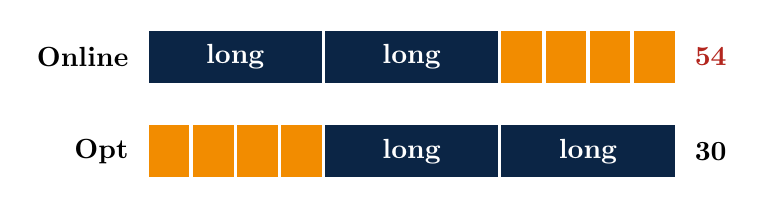
\begin{tikzpicture}[x=0.56cm,y=1cm]
    \onslide<2->{
      \node[anchor=east,font=\bfseries] at (-0.2,1.85) {Online};
      \gbar{0}{4}{1.5}{lng}{long}\gbar{4}{8}{1.5}{lng}{long}
      \foreach \i in {8,9,10,11} {\gbar{\i}{\i+1}{1.5}{sht}{}}
      \node[anchor=west,red] at (12.2,1.85) {$\mathbf{54}$};
    }
    \onslide<3->{
      \node[anchor=east,font=\bfseries] at (-0.2,0.65) {\Opt};
      \foreach \i in {0,1,2,3} {\gbar{\i}{\i+1}{0.3}{sht}{}}
      \gbar{4}{8}{0.3}{lng}{long}\gbar{8}{12}{0.3}{lng}{long}
      \node[anchor=west] at (12.2,0.65) {$\mathbf{30}$};
    }
  \end{tikzpicture}

  \vspace{2mm}
  \onslide<2->{\inclass{as in paging, the adversary answers our own choice}}

  \vspace{2mm}
  \onslide<4->{\keybox{Theorem (one machine).}{Every deterministic\\ algorithm has competitive ratio at least $\sqrt{\lambda}$.}}
\end{frame}

% ======================================================================
\begin{frame}{Starting at once can be very bad}
  \centering
  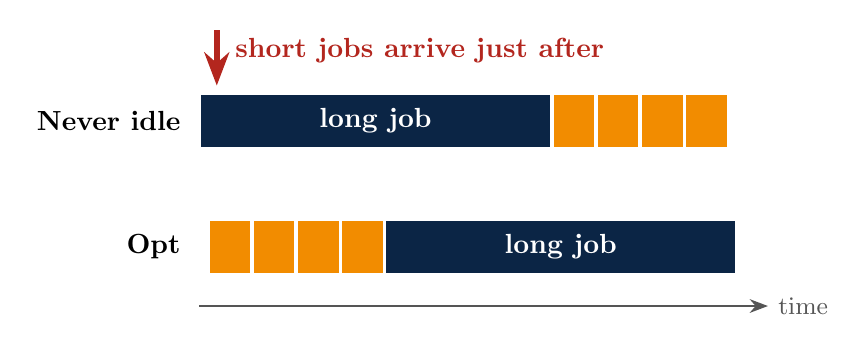
\begin{tikzpicture}[x=0.56cm,y=1cm,>=Stealth]
    \node[anchor=east,font=\bfseries] at (-0.2,2.45) {Never idle};
    \gbar{0}{8}{2.1}{lng}{long job}
    \onslide<2->{
      \draw[->,red,line width=2pt] (0.4,3.6) -- (0.4,2.9);
      \node[anchor=west,red,font=\bfseries] at (0.6,3.35) {short jobs arrive just after};
      \foreach \i in {8,9,10,11} {\gbar{\i}{\i+1}{2.1}{sht}{}}
    }
    \onslide<3->{
      \node[anchor=east,font=\bfseries] at (-0.2,0.85) {\Opt};
      \foreach \i in {0,1,2,3} {\gbar{\i+0.2}{\i+1.2}{0.5}{sht}{}}
      \gbar{4.2}{12.2}{0.5}{lng}{long job}
    }
    \draw[->,thick,gray] (0,0.1) -- (12.9,0.1) node[right,font=\small] {time};
  \end{tikzpicture}

  \vspace{3mm}
  \onslide<4->{\keybox{Observation.}{A rule that never idles has an\\ \textbf{unbounded} competitive ratio.}}

  \vspace{2mm}
  \onslide<5->{This covers FCFS and shortest limit first.}
\end{frame}

% ======================================================================
\begin{frame}{Idea: wait, but not too long}
  Take the job with the smallest limit.\\ Start it only when \ $t \ge \alpha \cdot u_j$.
  \vspace{1mm}

  \onslide<2->{\inclass{ski rental. Rent (wait) or buy (start)?\\ Break-even balances the two costs.}}
  \vspace{1mm}

  \centering
  \renewcommand{\arraystretch}{1.15}
  \begin{tabular}{c@{\quad\ }c@{\quad\ }c}
    \toprule
    $\alpha$ & waiting costs & blocking costs \\
    \midrule
    \uncover<3->{$1$} & \uncover<3->{{\color{red}$\boldsymbol{\lambda}$}} & \uncover<3->{$1$} \\
    \uncover<4->{$1/\lambda$} & \uncover<4->{$1$} & \uncover<4->{{\color{red}$\boldsymbol{\lambda}$}} \\
    \uncover<5->{$\boldsymbol{1/\sqrt{\lambda}}$} & \uncover<5->{$\boldsymbol{\sqrt{\lambda}}$} & \uncover<5->{$\boldsymbol{\sqrt{\lambda}}$} \\
    \bottomrule
  \end{tabular}

  \vspace{2mm}
  \onslide<6->{\keybox{Conjecture.}{With $\alpha = 1/\sqrt{\lambda}$ the rule is $(1 + \sqrt{\lambda})$-competitive.}}
\end{frame}

% ======================================================================
\begin{frame}{Experiment: the worst ratio we found}
  \centering
  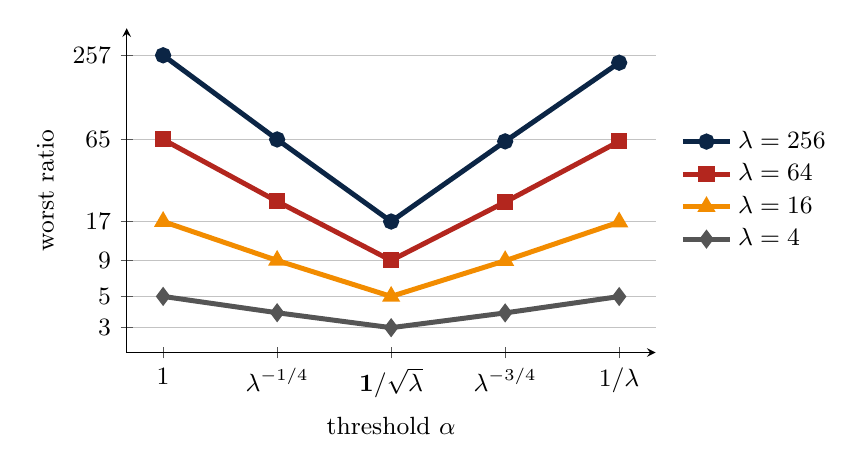
\begin{tikzpicture}
    \begin{axis}[width=8.3cm,height=5.7cm,ymode=log,axis lines=left,clip=false,
        xmin=-0.08,xmax=1.08,ymin=2,ymax=400,
        xtick={0,0.25,0.5,0.75,1},
        xticklabels={$1$,$\lambda^{-1/4}$,$\mathbf{1/\sqrt{\lambda}}$,$\lambda^{-3/4}$,$1/\lambda$},
        ytick={3,5,9,17,65,257},yticklabels={3,5,9,17,65,257},
        ymajorgrids,grid style={gray!35},
        xlabel={threshold $\alpha$},ylabel={worst ratio},
        tick label style={font=\small},label style={font=\small},
        legend style={draw=none,font=\small,at={(1.03,0.5)},anchor=west},
        legend cell align=left]
      \addplot[navy,line width=1.8pt,mark=*] coordinates {(0,257) (0.25,65) (0.5,17) (0.75,62.98) (1,227.75)};
      \addplot[red,line width=1.8pt,mark=square*] coordinates {(0,65) (0.25,23.63) (0.5,9) (0.75,23.36) (1,62.96)};
      \addplot[orange,line width=1.8pt,mark=triangle*] coordinates {(0,17) (0.25,9) (0.5,5) (0.75,8.96) (1,16.86)};
      \addplot[gray,line width=1.8pt,mark=diamond*] coordinates {(0,5) (0.25,3.83) (0.5,3) (0.75,3.82) (1,4.99)};
      \legend{$\lambda = 256$,$\lambda = 64$,$\lambda = 16$,$\lambda = 4$}
    \end{axis}
  \end{tikzpicture}

  \vspace{1mm}
  \onslide<2->{Best at $\alpha = 1/\sqrt{\lambda}$. The worst ratio there is $1 + \sqrt{\lambda}$: \ 3, 5, 9, 17.}

  \onslide<3->{{\small\color{navy}\textbf{In progress:} a proof. An experiment is not an upper bound.}}
\end{frame}

% ======================================================================
\section{Next step}

\begin{frame}{Machines are not the same}
  \begin{itemize}
    \item<1-> Real clusters mix machines: CPU and GPU nodes, old and new cloud instance types.
  \end{itemize}
  \vspace{1mm}
  \centering
  \onslide<2->{
  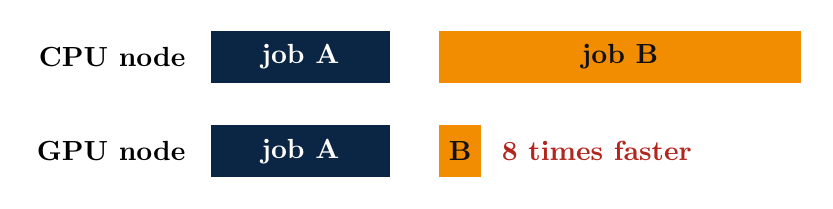
\begin{tikzpicture}[x=0.58cm,y=1cm]
    \node[anchor=east,font=\bfseries] at (-0.3,1.95) {CPU node};
    \node[anchor=east,font=\bfseries] at (-0.3,0.75) {GPU node};
    \gbar{0}{4}{1.6}{lng}{job A}
    \gbar{0}{4}{0.4}{lng}{job A}
    \onslide<3->{
      \gbar{5}{13}{1.6}{sht}{job B}
      \gbar{5}{6}{0.4}{sht}{B}
      \node[anchor=west,red,font=\bfseries] at (6.2,0.75) {8 times faster};
    }
  \end{tikzpicture}}

  \vspace{1mm}
  \begin{itemize}
    \item<4-> Job $j$ on machine $i$ runs for \ $p_j / s_{ij}$.
    \item<5-> The speeds $s_{ij}$ are known. \ $p_j$ is still hidden.
  \end{itemize}
\end{frame}

% ======================================================================
\begin{frame}{A new decision: which machine?}
  \centering
  \begin{tikzpicture}[x=0.7cm,y=1cm,>=Stealth]
    \node[anchor=east,font=\bfseries] at (-0.2,2.95) {Fast};
    \node[anchor=east,font=\bfseries] at (-0.2,0.75) {Slow};
    \gbar{0}{3}{2.6}{lng}{busy}
    \draw[pattern=north east lines,pattern color=navy,draw=navy,line width=1pt] (3,2.6) rectangle (9,3.3);
    \node[fill=white,inner sep=2pt,font=\small] at (6,2.95) {ends somewhere here};
    \draw[->,red,line width=2pt] (1,4.3) -- (1,3.5);
    \node[anchor=west,red,font=\bfseries] at (1.2,4.05) {a new job arrives};
    \only<2>{
      \gbar{1}{7}{0.4}{sht}{slow machine, now}
    }
    \only<3->{
      \gbar{1}{7}{0.4}{ghost}{slow machine, now}
      \gbar{9}{10.5}{2.6}{sht}{}
      \node[anchor=west,font=\bfseries] at (10.6,2.95) {wait};
      \draw[<-,red,line width=2pt] (3.1,2.3) -- (8.9,2.3);
      \node[font=\small] at (6,1.9) {earlier, if the fast machine frees up sooner};
    }
    \draw[->,thick,gray] (0,0.1) -- (11.6,0.1) node[right,font=\small] {time};
  \end{tikzpicture}

  \vspace{3mm}
  \onslide<4->{\textbf{The slow machine now, or the fast one later?}}

  \vspace{1mm}
  \onslide<5->{{\small\color{navy}\textbf{Future work:} how does the competitive ratio depend on the speed differences?}}
\end{frame}

% ======================================================================
\section{Conclusion}

\begin{frame}{Summary}
  \begin{itemize}\setlength{\itemsep}{2mm}
    \item<1-> \textbf{What:} schedule jobs online when we know only their time limits. Minimize $\sum_j C_j$.
    \item<2-> \textbf{Why:} real clusters work this way, and the limits are weak hints.
    \item<3-> \textbf{Course:} bin packing with an order, with waiting (ski rental), and with hidden sizes.
    \item<4-> \textbf{So far:} lower bound $\sqrt{\lambda}$; \ a waiting rule that reaches $1 + \sqrt{\lambda}$ in experiments. \ {\color{navy}Proof in progress.}
    \item<5-> \textbf{Next:} machines with different speeds.
  \end{itemize}
  \vspace{2mm}
  \centering
  \onslide<5->{{\color{navy}\bfseries\Large Questions?}}
\end{frame}

\end{document}
